\documentclass[a4paper,12pt]{article} % тип документа

% report, book



%  Русский язык

\usepackage[T2A]{fontenc}			% кодировка
\usepackage[utf8]{inputenc}			% кодировка исходного текста
\usepackage[english,russian]{babel}	% локализация и переносы
\usepackage{graphicx}
\graphicspath{{./}}
\DeclareGraphicsExtensions{.png,.jpg}


% Математика
\usepackage{amsmath,amsfonts,amssymb,amsthm,mathtools} 


\usepackage{wasysym}

%Заговолок
\author{Бредихин Александр}
\title{Домашняя работа №6}



\begin{document} % начало документа
\maketitle
\subsection*{Задача 1}
\textit{Задача:} дано $n$ слов длины $k$, состоящих из маленьких букв латинского алфавита. Предложите эффективный алгоритм их сортировки в лексикографическом (словарном) порядке.\\

\textit{Алгоритм:} используем <<radix sort>>: \\
начинаем с начала слов и сортируем поразрядно с помощью сортировки подсчётом (так как букв конечное число, то можем считать вхождение каждой, а затем выводить слова в нужном порядке по первому разряду). Затем аналогично сортируем по второму разряду, но с учётом результата сортировки по первому (то есть внутри каждого из подмножеств слов равных по сравнению предыдущих разрядов).\\
Если слова разной длины, то меньшие по длине слова дополняем символом, которые считаем меньше любой из буквы и тогда сортировка подсчётом не нарушается (в задаче сказано, что все слова одинаковой длины, поэтому этот пункт не важен).\\

\textit{Корректность:} поразрядно сортируем начиная с самого левого элемента с помощью сортировки подсчёта $ \longrightarrow $ получаем лексикографический порядок.\\

\textit{Сложность:} Сортировка подсчётом выполняется за $\mathcal{O}(n)$ (так как просто считает количество вхождений букв, а затем выводит их в нужном порядке). Она выполняется $ k $ раз. Следовательно сложность нашего алгоритма: $ \mathcal{O}(n \cdot k) $
  
  
  
\subsection*{Задача 2}
\textit{Задача:} пусть числовой массив $a[1],\dots,a[n]$ строго унимодален на максимум. Это означает, что существует $t$, такое что
$$
a[1]<a[2]<\dots< a[t]> a[t+1]>\dots> a[n-1]> a[n],
\quad 1\leq t\leq n.
$$
Разрешается за один ход спросить значение одного элемента массива.
Докажите, что можно найти значение максимального элемента $a[t]$ за
не более $O(\log n)$ ходов.\\

\textit{Алгоритм:} рассматриваем элемент $ a \left[\left[\frac{n}{2}\right]\right] $ (спрашиваем его значение). Спрашиваем значения соседних элементов $ a \left[\left[\frac{n}{2} - 1\right]\right] $ и $ a \left[\left[\frac{n}{2} + 1\right]\right] $ (дальше округления не пишутся, потому что не влияют на понимание алгоритма). Сравниваем центральный и левый от него элемент: если $ a \left[\frac{n}{2} - 1\right] > a \left[\frac{n}{2}\right] $, то применяем алгоритм к левой части, если $ a \left[\frac{n}{2} - 1\right] < a \left[\frac{n}{2}\right] $, то сравниваем: если $ a \left[\frac{n}{2} \right] < a \left[\frac{n}{2} + 1\right] $, то запускаем алгоритм от правой части, если $ a \left[\frac{n}{2}\right] > a \left[\frac{n}{2} + 1\right] $, то элемент $ a \left[\frac{n}{2}\right] $ искомый и алгоритм завершается.\\

\textit{Корректность:} алгоритм завершается только тогда  когда оба его соседа меньше него, так как массив унимодален на максимум, то этот элемент обязан быть максимальным во всём массиве.\\

\textit{Сложность:} на каждом из шагов делаем константное количество запросов (узнаём 3 элемента: центральный элемент подмассива и его соседей). С каждом шагом длина массива уменьшается вдвое, следовательно, глубина рекурсии $ \log(n) $, тогда сложность алгоритма:  $ \mathcal{O}(\log n) $
  
\subsection*{Задача 3}
\textit{Задача:} имеется $n$ монет, среди которых одна фальшивая, и чашечные весы.
Настоящие монеты все имеют одинаковый вес, а фальшивая легче. На каждую чашку весов можно класть произвольное количество монет.
Докажите, что фальшивую монету можно найти за $\log_3 n+c$ взвешиваний.\\

\textit{Алгоритм:} разбиваем все монеты на 3 равные части (если это не получается, то есть если $ n $ не делится без остатка на 3, то могут остаться либо 1, либо 2 монеты не в одной из куч). \\
Кладём на весы первую и вторую кучу. Если они равны, то фальшивая монета либо в 3ей куче, либо она одна из отложенных монет, а в 1ой и во 2ой куче все монеты настоящие (так как фальшивая монета только одна, а остальные одинакового веса). Берём монету из 1ой кучи и сравниваем её с отложенными, если какая-то из них оказалась меньше, то она фальшивая и мы заканчиваем выполнение алгоритма, если они равны, то фальшивая монета будет лежать в 3ей кучи и мы делаем все эти действия для неё.\\
Если какая-то из куч (1ая или 2ая) оказалась меньшая по весу, то повторяем описынные действия для неё.\\
Останавливаемся либо когда нашли фальшивую монету на каком-то из шагов, либо когда размер кучи станет 1 (тогда эта монета будет фальшивой).\\

\textit{Корректность:} из алгоритма следует, что на каждом шаге просматриваем все монеты и корректно выбираем то, множество, где она есть. Алгоритм остановится, так как количество монет-претендентов на фальшивую уменьшается с каждым шагом.\\

\textit{Сложность:} на каждом шаге производим константное количество взвешиваний: в худшем случае 3. С каждым шагом уменьшаем размер кучи в 3 раза, следовательно, максимальная глубина рекурсии $ \log_3(n) $. Следовательно сложность алгоритма: $ \mathcal{O}(\log_3 n+c) $


\subsection*{Задача 4}
\textit{Задача:} докажите, что в условиях предыдущей задачи для нахождения фальшивой
монеты необходимо $\log_3 n + c$ взвешиваний.\\

Расмотрим триарное полное дерево. Считаем, что монета фальшивая, если спускаясь по этому дереву мы спустились в лист с монетой где записано, что она фальшивая, а листья дерева это взвешивания из которых идут три ребра в зависимости от результата взвешивания. Нужно, чтобы дерево выдавало ответ задачи на любую из монет (иначе мы можем её переставить с фальшивой и ответ не изменится $ \longrightarrow $ станет неправильным), следовательно, у этого дерева долно быть $ \geq n $ листьев. У полного триарного дерева на $ k $ом уровне $ 3^k $ листьев, следовательно $ k \geq \log_3(n) $ (следовательно, необходимо $ \geq log_3(n) + c $ взвешиваний).


\subsection*{Задача 5}
\textit{Задача:} даны два отсортированных массива длины $n$. Предложите как можно более эффективный алгоритм поиска медианы в массиве, состоящем из всех данных $2n$ элементов. Можно считать, что все элементы различные. Докажите корректность алгоритма и оцените его сложность (количество сравнений). В этой задаче обращения к элементам массива выполняются за O(1), читать оба массива целиком не требуется, считайте, что они уже лежат в памяти.\\

Пусть два отсортированных массива называются A и B. Чтобы найти медиану общего массива разобьём массивы в местах $ i $ и $ j $, тогда медиана общего массива эквивалента следующим условиям: 
$$
1) \quad i + j = 2n - i - j + 2
$$
$$
2) \quad B[j - 1] \leq A[i] \quad and \quad A[i - 1] \leq B[j]
$$
Первое условие гарантирует, что это медиана (учитываем индексацию с 0). Установим $ imin = 0, imax = n $ и начнём бинарным поискам искать значение $ i $, так чтобы предыдущие 2 условия удволетворялись:\\
пусть $ i = \frac{imin + imax}{2}, j = \frac{2n + 1}{2} - i $ (этим мы удволетворили первое словие, что длины левой и правой части равны). Возможны 3 ситуации:
\begin{itemize}
\item[1)] если $ \quad B[j - 1] \leq A[i] \quad and \quad A[i - 1] \leq B[j] $, то мы нашли нужный $ i $ и можем прекращать поиск.
\item[2)] если $ B[j - 1] > A[i] $, значит мы должны увеличить $ i $, чтобы $ B[j - 1] \leq A[i] $, смотреть условие 2. Мы не можем уменьшать $i$, так как тогда $ j $ возрастёт, следовательно, возрастёт и $ B[j-1] $, а $ A[i] $ уменьшится, что отдалит нас от достижения нужного неравенства.
\item[3)] $ A[i - 1] > B[j] $, мы должны уменьшить $ i $, чтобы выполнилось нужное неравенство $ A[i - 1] \leq B[j] $ (по аналогичным пункту 2 рассуждениям $ i $ в этом случае нельзя увеличивать).
\end{itemize} 
Увеличиваем или уменьшаем $ i $ бинарно, то есть начинаем искать нужный $ i $ передвигая границы: для второго пункта $ imin = i + 1 $, для 3го: $ imax = i - 1 $. Повторяем операции заново (смотреть с установления нового $ i $).\\
Останавливаемся, если нашли нужный $ i $ или он стал $ 0 $ или $ n $. Тогда медианой массива будет являться элемент $\frac{max \left( A[i - 1], B[j - 1] \right) + min \left( A[i], B[j] \right) }{2}  $.\\

\textit{Корректность:} из алгоритма следует, что на каждом шаге мы отбрасываем рассмотрение расположений индекса, которые не удволетворяют условию 1,2 (в алгоритме объяснено почему), которые показывают, что все элементы слего него меньше и их половина. Алгоритм остановится, так как на каждом шаге диапазон возможных положений $ i $ уменьшается.\\

\textit{Сложность:} На кажом шаге уменьшаем диапозон возможных расположений $ i $ а два раза (как в бинарном поиске). Первоначально он равен $ n $, следовательно, в худшем случае потребуется $ \log(n) $ шагов, на каждом из которых проделываем сравнения элементов сложность которых $ \mathcal{O}(1) $. Значит, сложность алгоритма:  $ \mathcal{O}(\log(n)) $ 



\subsection*{Задача 6}
\textit{Задача:} определите, что число является значением данного многочлена с натуральными коэффициентами в натуральной точке. На вход задачи подаются натуральные числа $n, a_0, \ldots a_n$ и $y$. Необходимо определить, существует ли натуральное число $x$, такое что $$ y = a_n x^n + a_{n-1} x^{n-1} + \ldots + a_1x +  a_0. $$\\

Перенесём свободный коэффициент многочлена $ a_0 $ влево, получим:
$$ y - a_0 = a_n x^n + a_{n-1} x^{n-1} + \ldots + a_1x . $$
Правая часть делится на $ x $, следовательно левая тоже делится на $ x $. Начинаем перебирать значения $ x $ от 1 до $A = y - a_0 $. Проверяя, является ли оно делителем $ A $, если является, то подставляем в многочлен и проверяем значение в этой точке совпадает оно с $ y $ или нет (если не в какой из точек не было достигнуто равенство, то натуральных решений нет). Считаем значение в какой-то конкретной точке с помощью схемы Горнера, которая представляет наш многочлен в виде:
$$
P_{n}(x)=\left(\ldots\left(\left(a_{0} x+a_{1}\right) x+a_{2}\right) x+\ldots+a_{n-1}\right) x+a_{n}
$$
Поэтому для вычисления многочлена, которое проводится в порядке, как стоят скобки, потребуется $ n $ умножений и $ n-k $ сложений, где $ k $ количество коэффициентов многочлена равных 0).\\
Проверка на делимость осуществляется за $\mathcal{O}(\log(A)) $ (проверяем равен ли НОД(A,x) = $ x $, где $ x $ -- предполагаемый делитель). В итоге общая сложность алгоритма: $\mathcal{O}(n \cdot A \cdot \log(A)) $, где $ A = y-a_0 $.\\
Корректность алгоритма следует из правил математики (сокращаем полный перебор, проверяя на делимость) 


\subsection*{Задача 7}
\textit{Задача:} ваш лектор по алгоритмам нашёл два одинаковых прочных шарика из неизвестного материала и внезапно решил измерить их прочность в этажах стоэтажного небоскрёба: прочность равна номеру минимального этажа, при броске шарика из окна которого шарик разобъётся (максимум 100). Считаем, что если шарик уцелел, то его прочность после броска не уменьшилась. Сколько бросков шариков необходимо и достаточно для нахождения прочности?\\

Заметим, что если один из шариков разобьётся, то другой мы должны бросать на каждом этаже, начиная с того, для которого мы уже проверили, что не разбивается. Построим дерево для которого: левая ветвь показывает этаж, с которого нужно бросать, если первый шарик разбился на данном броске, правая -- если не разбился. Это дерево имеет такой вид: 
\begin{center}
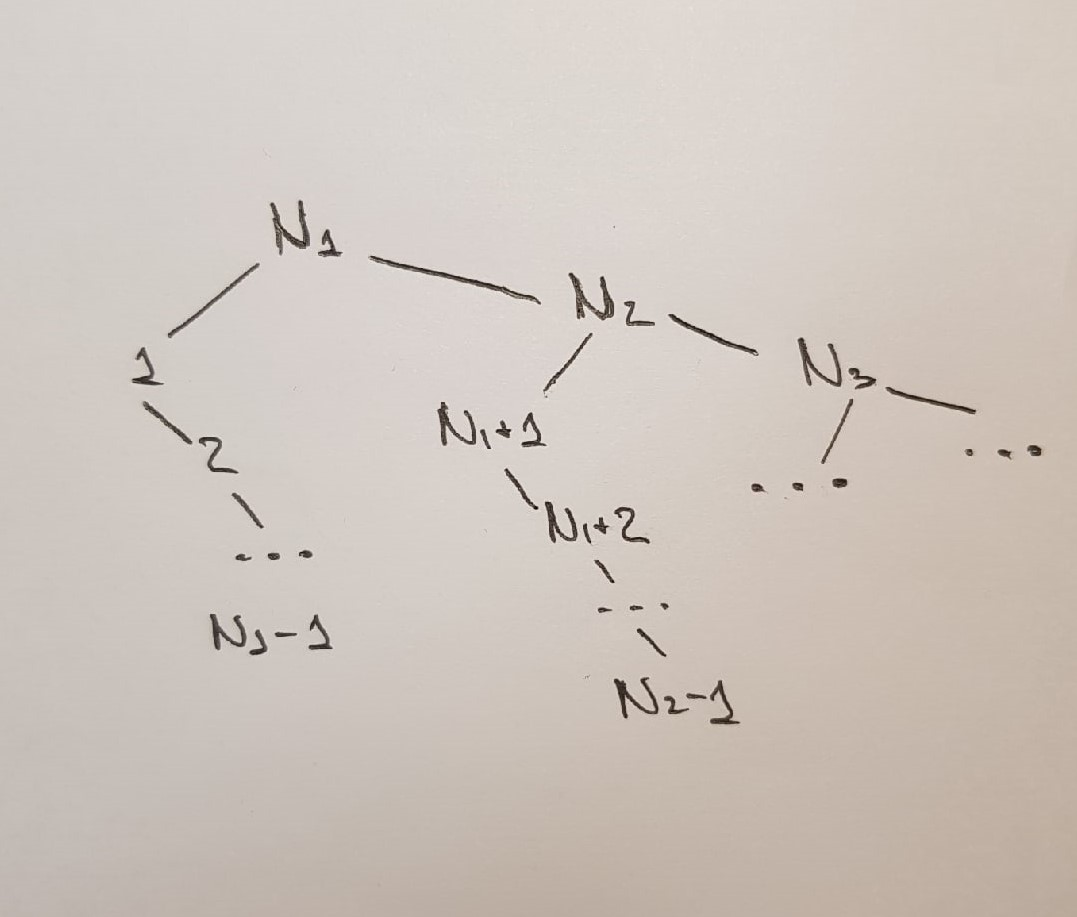
\includegraphics[width=0.7\textwidth]{tree_7}
\end{center}
Нам нужно подобрать $N_1, \quad N_2, \quad \ldots $ так, чтобы все ветки имели одинаковую длину и она была как можно меньше. Запишем равенство ветвей дерева (количество бросков для каждой из ветки дерева):
$$
\begin{aligned}
&N_{1}=N_{2}-N_{1}+1\\
&N_{2}-N_{1}=N_{3}-N_{2}+1\\
& \ldots \\
&N_{n-1}-N_{n-2}=N_{n}-N_{n-1}+1
\end{aligned}
$$
Подставляем первое уравнение во второе, второе в первое и так далее, получаем: 
$$
N_{n}=N_{n-1}+N_{1}-(n-1)
$$
В этом уравнение заменим $ n $ на $ n - 1 $ и подставим в это же и так далее, тогда получим следующую зависимость:
$$
N_{n}=n \cdot N_{1}-(n-1)-(n-2)-(n-3)-\ldots=n \cdot N_{1}-\frac{(n-1) n}{2}
$$
В ней:  $ N_n $ -- необходимый нам этаж. $ N_1 $ -- этаж, с которого мы сбрасываем первый шарик. Зафиксируем его и найдем при каком $ n $ мы сможем достичь максимально нужного нам этаже (в нашем случае $ N_{max} = 100 $). Для этого берём производную у полученной зависимости, считая её как непрерывную функцию от $ n $: 
$$
\frac{d N(n)}{d n}=N_{1}-n+\frac{1}{2}=0
$$
$$
n_{\max }=N_{1}+\frac{1}{2}
$$
Подставляем это значение в уравнение и приравниваем к нашему максимальному этажу $ N_{max}$ и выражаем $ N_1 $:
$$
N\left(n_{\max }\right)=\frac{\left(N_{1}\right)^{2}}{2}+\frac{N_{1}}{2}=N_{max}
$$
$$
N_{1}=-\frac{1}{2}+\left(\frac{1}{4}+2 N_{\text {max}}\right)^{\frac{1}{2}}
$$
Подставляя значение  $ N_{max} = 100 $, находим $ N_1 = 14 $ (с округлением вверх). Так как мы делали так, что все ветки дерева равны, то число бросков, которое нужно сделать в худшем случае равно $ N_1 = 14 $.\\
Ответ: 14


\end{document} % конец документа